\documentclass[10pt,letterpaper]{article}
\usepackage[margin=0.88in,headheight=25pt]{geometry}
\usepackage[T1]{fontenc}
\usepackage[utf8]{inputenc}
\usepackage{lmodern,microtype,setspace,xcolor,titlesec,fancyhdr,hyperref}
\usepackage{tikz}
\usepackage{graphicx}
\usetikzlibrary{arrows.meta,positioning}
\definecolor{Periwinkle}{HTML}{727BE8}
\definecolor{Ink}{HTML}{101D39}
\definecolor{Mist}{HTML}{EEF0FC}
\hypersetup{colorlinks=true,urlcolor=Periwinkle,linkcolor=Periwinkle,pdftitle={SEFI Research Program: Organization Prospectus},pdfauthor={Jason Duran Dutton},pdfsubject={Independent research, scientific software, and academic collaboration}}
\setstretch{1.08}
\setlength{\parindent}{0pt}
\setlength{\parskip}{0.5em}
\titleformat{\section}{\Large\bfseries\color{Periwinkle}}{}{0pt}{}
\titleformat{\subsection}{\normalsize\bfseries\color{Ink}}{}{0pt}{}
\titlespacing*{\section}{0pt}{0pt}{12pt}
\titlespacing*{\subsection}{0pt}{10pt}{3pt}
\pagestyle{fancy}\fancyhf{}
\fancyhead[L]{\sffamily\bfseries\color{Ink}SEFI\enspace{\scriptsize\color{Periwinkle}RESEARCH PROGRAM}}
\fancyhead[R]{\sffamily\scriptsize\color{Ink}ORGANIZATION PROSPECTUS}
\fancyfoot[L]{\footnotesize Jason Duran Dutton\enspace|\enspace Castlewood, Virginia}
\fancyfoot[R]{\sffamily\small\color{Periwinkle}\thepage}
\renewcommand{\headrulewidth}{0.4pt}
\newcommand{\pageheading}[2]{\clearpage\section{#1}\textit{#2}\par\medskip}
\newcommand{\statement}[1]{\par\medskip\begingroup\color{Periwinkle}\hrule\smallskip\color{Ink}#1\par\smallskip\color{Periwinkle}\hrule\endgroup\medskip}
\setlength{\emergencystretch}{1.5em}
\tikzset{panel/.style={draw=Periwinkle!55,fill=Mist,rounded corners=3pt,align=center,font=\sffamily\footnotesize,text=Ink,minimum height=0.47in,text width=1.31in,inner sep=5pt},flow/.style={-{Stealth[length=4pt]},thick,draw=Periwinkle}}
\newcounter{programfigure}
\newcommand{\figurecaption}[2]{\refstepcounter{programfigure}\par\smallskip{\footnotesize\color{Periwinkle}\textbf{Figure \theprogramfigure. #1}\enspace\color{Ink}#2\par}}
\begin{document}
\color{Ink}
\thispagestyle{empty}
\noindent\begin{minipage}[c]{0.17\linewidth}

\begin{tikzpicture}[x=1cm,y=1cm]
\fill[Ink] (0,0) rectangle (1.65,1.65);
\foreach \angle in {0,60,120}{
\draw[Periwinkle,line width=0.8pt,rotate around={\angle:(0.825,0.825)}] (0.825,0.825) ellipse (0.63 and 0.26);
}
\fill[cyan!55!white] (0.825,0.825) circle (0.10);
\fill[white] (1.455,0.825) circle (0.065);
\end{tikzpicture}
\end{minipage}\hfill
\begin{minipage}[c]{0.81\linewidth}
{\sffamily\fontsize{38}{41}\selectfont\bfseries\color{Ink}SEFI}\par
\vspace{3pt}
{\sffamily\small\bfseries\color{Ink}R E S E A R C H\quad P R O G R A M}
\end{minipage}\par
\vspace{0.12in}
{\sffamily\fontsize{7.5}{9}\selectfont\color{Periwinkle}COMPUTATIONAL SCIENCE\quad /\quad PHYSICS\quad /\quad QUANTUM INFORMATION}\par
{\color{Periwinkle}\hrule height 1.5pt}
\vspace{0.06in}
\noindent\begin{minipage}[t]{0.48\linewidth}
{\sffamily\fontsize{8}{10}\selectfont 1009 High Point Road\\Castlewood, Virginia 24224, United States}
\end{minipage}\hfill
\begin{minipage}[t]{0.49\linewidth}
{\sffamily\fontsize{8}{10}\selectfont\textbf{JASON DURAN DUTTON}\\Student, American InterContinental University\\\href{mailto:Jason.Dutton7@student.aiuonline.edu}{Jason.Dutton7@student.aiuonline.edu}\\(276) 210-4696}
\end{minipage}\par
\vspace{0.2in}
{\sffamily\fontsize{21}{25}\selectfont\bfseries Organization Prospectus}\par
{\small Founder and Supervising Researcher: Jason Duran Dutton}\par
\vspace{0.12in}
\section{Executive Summary}
SEFI Research Program is an independent research initiative directed by Jason Duran Dutton, founder and supervising researcher and a student enrolled at American InterContinental University (AIU). The program brings scientific software development, computational investigation, and manuscript preparation into a continuing body of work spanning computational physics, scientific computing, photonics, quantum information, and mathematical modeling.

This prospectus has a specific academic purpose: to connect Dutton's enrollment at AIU with the research he is developing through SEFI. He seeks a constructive pathway through which his software, manuscripts, and computational investigations can inform his academic development and receive faculty guidance and scholarly evaluation. The portfolio includes SEFI-PY, the SEFI QEC Stack, geometric photonic quantum error-correction research, scientific solver development, and calibration and diagnostic systems.

SEFI's mission is to advance scientific understanding through computational tools, mathematical models, reproducible workflows, and accessible technical resources. Its research philosophy connects practical engineering habits with mathematical analysis and scientific programming. For Dutton, university study and independent research are mutually reinforcing activities: academic learning can strengthen the work's foundations, while research provides concrete problems through which to deepen and demonstrate understanding.

The proposed connection begins with review of a defined research portfolio and discussion with appropriate AIU advisors or faculty about suitable academic opportunities. Any supervised project, course connection, or formal arrangement would require university agreement. The present relationship is Dutton's enrollment; SEFI remains independently directed. This document offers the research for consideration and identifies a practical basis for developing that relationship.

\pageheading{Organizational Identity and Mission}{A continuing framework for independent scientific work}
SEFI Research Program provides an organizational home for research that crosses the boundaries between software engineering, applied mathematics, and physical modeling. Individual repositories and manuscripts can address distinct problems while contributing to a common research agenda. The program supplies continuity: methods developed in one project can be examined in another, documentation can follow shared standards, and research questions can persist beyond the completion of a single implementation.

Its identity rests on the relationship between scientific questions and concrete artifacts. A model becomes useful when its assumptions are explicit and its consequences can be examined. A software system becomes a scientific contribution when its behavior is documented and its results can be interpreted. A manuscript becomes more valuable when readers can trace its computational claims to an identifiable implementation. SEFI seeks to develop these elements together so that each strengthens the others.

Dutton's enrollment at American InterContinental University provides the immediate academic context for this prospectus. He intends to connect the program's research with his education through relevant learning objectives, faculty feedback, and opportunities for supervised inquiry. This connection concerns his development as a student and researcher; any institutional role would be established through a separate agreement with AIU.

The mission is to advance understanding through the development of computational tools, mathematical models, reproducible workflows, and openly accessible resources. In practice, this means selecting questions with a defined scope, constructing implementations that expose the relevant assumptions, examining results against appropriate references, and communicating both findings and limitations. The program's ambitions extend across several disciplines, but individual projects must remain specific enough to support meaningful evaluation.

Four connected pillars organize this work. Scientific computing supplies the software and numerical foundations. Computational physics connects those foundations to representations of physical systems. Photonics and quantum information provide a focused domain for investigating state evolution, error behavior, and correction concepts. Open research infrastructure connects implementations, records, and publications so that the work can be understood beyond the environment in which it was produced.

These pillars describe related responsibilities within a founder-led program. They provide a way to organize work and identify future collaborations; they do not imply separate staffed departments or independently equipped laboratories. Research divisions in this prospectus should be understood as areas of activity coordinated by the founder.

The program is based in Castlewood, Virginia. Its organizational value lies in sustained stewardship of research questions, software, and technical writing. As the portfolio develops, SEFI intends to preserve a recognizable standard of care across these outputs: clear scope, inspectable methods, qualified conclusions, and sufficient documentation to support further inquiry.

\begin{center}
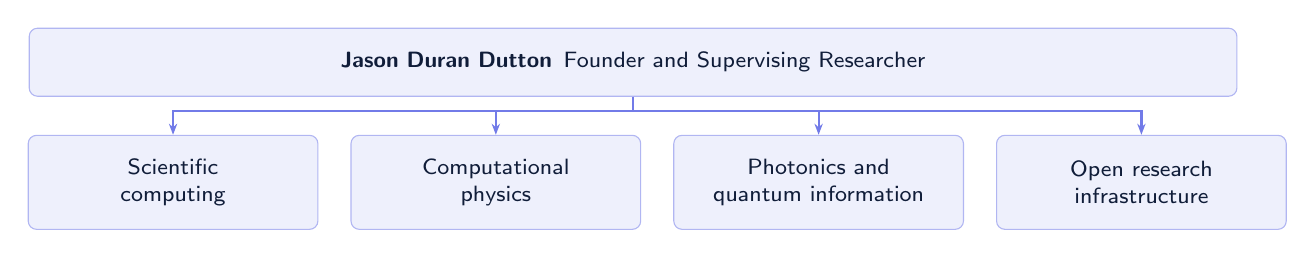
\begin{tikzpicture}[node distance=0.16in]
\node[panel,text width=5.9in,minimum height=0.34in] (lead) {\textbf{Jason Duran Dutton}\enspace Founder and Supervising Researcher};
\node[panel,below=0.19in of lead,xshift=-2.3in] (a) {Scientific\\computing};
\node[panel,right=0.16in of a] (b) {Computational\\physics};
\node[panel,right=0.16in of b] (c) {Photonics and\\quantum information};
\node[panel,right=0.16in of c] (d) {Open research\\infrastructure};
\draw[flow] (lead.south) -- ++(0,-0.07in) -| (a.north);
\draw[flow] (lead.south) -- ++(0,-0.07in) -| (b.north);
\draw[flow] (lead.south) -- ++(0,-0.07in) -| (c.north);
\draw[flow] (lead.south) -- ++(0,-0.07in) -| (d.north);
\end{tikzpicture}
\figurecaption{Program structure}{Research responsibilities within a founder-led program; boxes denote areas of work, rather than separate staffed departments.}
\end{center}

\statement{\textbf{Mission}\quad Advance scientific understanding by building computational tools and mathematical models whose assumptions, methods, and results can be examined, reproduced, and improved.}

\pageheading{Founder and Research Leadership}{Engineering experience translated into computational inquiry}
Jason Duran Dutton is the founder and supervising researcher of SEFI Research Program. His technical background, as described in the supplied biographical materials, includes electrical and mechanical systems, commissioning support, instrumentation, controls verification, maintenance supervision, diagnostics, and industrial troubleshooting. This experience provides a practical foundation for the program's approach to scientific problem solving.

Work in complex technical environments requires more than identifying a plausible explanation. A diagnosis must account for observed behavior, distinguish causes from symptoms, and survive further measurement. A correction must be checked under the conditions that produced the original problem. These habits are directly relevant to computational investigation, where an attractive result can arise from an implementation defect, an unsuitable assumption, or a poorly chosen comparison.

Dutton's movement toward mathematics, physics, and scientific computing developed through independent study, software construction, numerical experimentation, and technical writing. Within SEFI, programming provides a means of giving mathematical ideas an operational form. Models can be implemented, assumptions varied, and computational behavior examined in ways that support a more precise understanding of the original question.

The founder's role combines scientific direction with responsibility for implementation and communication. This includes identifying research problems, developing software, interpreting computational results, maintaining technical documentation, and preparing manuscripts. Bringing these activities together creates a close relationship between an argument and the software used to investigate it. It also makes careful review especially important, because the same person may originate a concept, implement it, and assess the outcome.

SEFI's response to that concentration of responsibility is to make the reasoning and evidence accessible to scrutiny. A convincing research record should allow another reader to identify what was assumed, what was computed, how the result was assessed, and what remains unresolved. Collaboration can strengthen this process by introducing independent mathematical analysis, implementation review, alternative benchmarks, and domain expertise.

Dutton is enrolled at American InterContinental University and seeks to make his research an intentional part of his academic development. He wants to bring a documented portfolio to advisors and faculty, identify where it connects with his studies, and establish appropriate opportunities for guidance and evaluation. Computational physics and scientific computing describe his research direction; they are not presented here as the title of his AIU degree program. Enrollment supplies an existing academic connection from which more focused engagement can develop.

The program's leadership model is therefore both practical and scholarly. Engineering experience informs how problems are approached, while scientific standards determine what conclusions the evidence can support. The intended result is a research environment in which persistence and technical capability are matched by intellectual discipline and openness to correction.

\pageheading{Scientific Computing and SEFI-PY}{The computational foundation of the research portfolio}
SEFI-PY is described in the program materials as SEFI's primary scientific computing framework. Its role is to connect numerical experimentation, data analysis, scientific visualization, computational prototyping, and validation workflows within a reusable software environment. It provides a common foundation for projects that would otherwise require repeated development of similar supporting tools.

The research value of a shared framework lies in the consistency it can bring to an investigation. A model implementation must interact with numerical methods, parameter choices, data structures, and reporting routines. When those relationships are explicit, researchers can examine how a change in one part of the workflow affects the result. When they are hidden in isolated scripts or undocumented manual steps, interpretation becomes more difficult.

SEFI-PY's intended architecture is modular. Model-specific components express the scientific assumptions of an investigation; numerical components perform the relevant computations; analysis routines examine the resulting data; and visualization and reporting tools communicate the outcome. This description establishes the organizing logic of the framework. Detailed statements about supported interfaces, dependencies, and implemented features should be tied to a particular software version.

Within the broader program, the framework supports a productive connection between exploratory work and more formal studies. Early implementations can help identify useful questions and reveal unexpected behavior. As a project matures, its inputs, procedures, and outputs can be made more explicit so that the investigation becomes repeatable. The transition requires documentation and review as well as code development.

Scientific computing also introduces its own research questions. Numerical choices can change stability, runtime, memory requirements, and the interpretation of apparent agreement. SEFI treats these properties as matters to investigate rather than background details. A computational tool should expose enough information for a researcher to understand whether a result depends on discretization, solver settings, stopping criteria, or other implementation decisions.

The framework's long-term value will depend on whether it supports useful work beyond its initial applications. Clear examples, documented assumptions, manageable dependencies, and identifiable releases can make individual components easier to evaluate and reuse. Growth should follow demonstrated needs within the research portfolio, preserving a coherent foundation as new capabilities are introduced.

SEFI-PY therefore occupies two roles. It is infrastructure for investigations in physics, mathematics, and diagnostics, and it is itself an evolving software contribution. Its success should be assessed through the clarity, reliability, and scientific usefulness of the workflows it enables.

\begin{center}
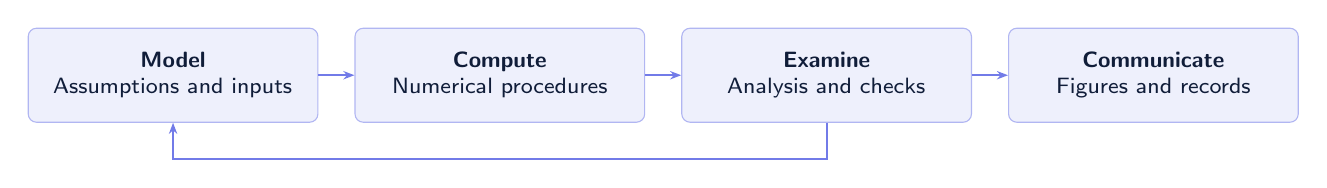
\begin{tikzpicture}[node distance=0.18in]
\node[panel] (a) {\textbf{Model}\\Assumptions and inputs};
\node[panel,right=of a] (b) {\textbf{Compute}\\Numerical procedures};
\node[panel,right=of b] (c) {\textbf{Examine}\\Analysis and checks};
\node[panel,right=of c] (d) {\textbf{Communicate}\\Figures and records};
\draw[flow] (a)--(b);\draw[flow] (b)--(c);\draw[flow] (c)--(d);
\draw[flow] (c.south) -- ++(0,-0.18in) -| (a.south);
\end{tikzpicture}
\figurecaption{SEFI-PY workflow}{Conceptual organization of a reproducible investigation. The return path represents refinement after analysis; it is not a verified software dependency map.}
\end{center}

\pageheading{Computational Physics and Numerical Research}{Physical models, solver development, and diagnostic systems}
Computational physics provides the central scientific orientation of SEFI Research Program. The work examines how mathematical representations of physical systems can be translated into computations and how the behavior of those computations informs the interpretation of the model. Relevant questions include dynamical evolution, geometric representations, field descriptions, numerical approximation, and stability.

A computational investigation begins with a physical or mathematical question and a set of assumptions. The implementation then creates an additional layer of choices: representation, resolution, approximation, and algorithm. SEFI's approach is to keep these layers visible. Agreement within a software implementation does not by itself establish that the underlying model captures the physical system of interest. Each connection requires its own reasoning and evidence.

\subsection{Scientific solver development}
The program materials identify sparse numerical methods and solver architectures as a research activity. This work concerns the relationship between computational structure and numerical behavior: how a problem can be represented efficiently, which operations dominate its cost, and whether an alternative implementation preserves an appropriate level of agreement with reference calculations.

The substantive output is a solver implementation accompanied by an interpretable account of its behavior. Performance comparisons need a defined problem family, consistent tolerances, stated computing conditions, and an explanation of what is being measured. A faster runtime is scientifically useful only in relation to accuracy, convergence, resource use, and the intended application. This prospectus does not assign a numerical advantage to a solver without the corresponding study.

\subsection{Calibration and diagnostic research}
Calibration and diagnostic systems connect the program's computational interests with the founder's engineering experience. The supplied materials describe frameworks for investigating drift, measurement interpretation, correction strategies, and recovery behavior. Such work can explore how a diagnostic decision changes when measurements are uncertain, model parameters vary, or a system evolves away from its initial condition.

The research contribution lies in making those relationships explicit and testable. A controlled computational scenario can isolate a source of drift or compare competing recovery strategies under shared assumptions. Its conclusions remain bounded by the scenario and model used. Application to an operating physical system would require suitable measurements and separate validation.

Together, physical modeling, solver development, and diagnostic analysis create a connected research strand. Physical questions motivate computational requirements; numerical work examines how those requirements can be met; and diagnostic reasoning helps interpret discrepancies. The resulting artifacts can include implementations, example problems, computational reports, and manuscripts that explain both the method and its limits.

\pageheading{Photonics and Quantum Information}{The SEFI QEC Stack and geometric research concepts}
Photonics and quantum information form a focused research domain within SEFI. The program materials describe investigations of optical mode evolution, stability, continuous-variable systems, error behavior, and geometric representations. These interests connect mathematical modeling with the development of software environments in which proposed relationships can be examined computationally.

\subsection{The SEFI QEC Stack}
The SEFI QEC Stack is described as a dedicated computational framework for quantum-information and photonic error-correction investigations. Its stated role includes error characterization, state evolution, correction and recovery workflows, and validation methods. It provides an organizational setting for translating research concepts into explicit computational procedures.

A useful study in this setting must define the represented state, the assumed evolution or noise process, the information available to a correction procedure, and the criterion used to assess the result. These definitions determine what a simulation can demonstrate. The stack's scientific value depends on how clearly its implemented operations correspond to the mathematical objects and physical assumptions of a particular investigation.

The framework can also support comparisons between a proposed method and a reference procedure. Such comparisons require a common task and compatible assumptions. Recovery performance, resource requirements, and sensitivity to model parameters should be interpreted together. A software experiment may establish behavior within a specified model while leaving physical feasibility and broader applicability open.

\subsection{Geometric photonic quantum error-correction research}
The supplied portfolio describes research involving worldline geometry, stability manifolds, error displacement, geometric correction mappings, and photonic mode evolution. These terms identify the program's conceptual direction. Their precise mathematical meanings, and their relationship to established quantum-information formalisms, must be supplied by the associated manuscripts and implementations.

The central opportunity is to investigate whether a geometric representation offers a useful way to characterize evolution or organize a correction problem. That question requires explicit definitions and testable consequences. A visual or geometric analogy can guide exploration, but a scientific claim needs a demonstrated correspondence between the representation, the operations performed, and the quantities being evaluated.

SEFI's prospectus presents this strand as an active area of computational and manuscript development. It does not treat proposed geometric descriptions as established physical mechanisms or claim experimental demonstration. Progress will be reflected in clearer formulations, reproducible examples, meaningful comparisons, and external review of the resulting arguments. These steps allow promising ideas to develop while keeping their evidentiary status visible.

\begin{center}

\begin{tikzpicture}[node distance=0.18in]
\node[panel] (a) {\textbf{Define}\\State and noise model};
\node[panel,right=of a] (b) {\textbf{Evolve}\\Simulated error process};
\node[panel,right=of b] (c) {\textbf{Recover}\\Candidate correction};
\node[panel,right=of c] (d) {\textbf{Assess}\\Metric and reference};
\draw[flow] (a)--(b);\draw[flow] (b)--(c);\draw[flow] (c)--(d);
\end{tikzpicture}
\figurecaption{QEC research workflow}{Conceptual study design. The correction stage depends on the information permitted by the stated model; this diagram reports no physical or performance result.}
\end{center}

\pageheading{Research Outputs and Publication Development}{A portfolio of software, manuscripts, and computational records}
SEFI's research portfolio is organized around identifiable outputs. SEFI-PY supplies shared scientific computing infrastructure. The SEFI QEC Stack provides a focused environment for quantum-information investigations. Geometric photonic research connects computational models with manuscript development. Solver and diagnostic projects extend the portfolio into numerical methods and engineering-informed analysis. Their relationship gives the program a more durable foundation than a collection of unrelated experiments.

\subsection{Software as a research contribution}
Research software embodies decisions that prose alone cannot fully convey. An implementation specifies operations, dependencies, data handling, and computational procedures. When those decisions are documented, the software allows others to inspect how a model was translated into a calculation and to explore whether the same method behaves differently under other conditions.

For that reason, the program's software outputs should be presented with a defined purpose and an identifiable scope. A project description should explain what question the software addresses, what a user can reproduce, and which limitations affect interpretation. Examples and release records can make the work easier to examine without requiring readers to reconstruct the development history.

\subsection{Manuscripts and technical writing}
The founding materials describe manuscript activity in computational physics, mathematical modeling, photonics, and quantum information. This prospectus treats those materials as a developing research portfolio. It does not supply publication titles, venues, acceptance decisions, or identifiers that were not provided. Drafting, public release, peer review, and formal publication are distinct stages that should be identified accurately in a final publication inventory.

The strongest relationship between software and writing is traceable. A manuscript explains the question, assumptions, method, and interpretation; the accompanying computational record identifies how relevant results were obtained. Where a paper makes a numerical claim, readers should be able to locate the inputs, procedure, and software version needed to examine it.

\subsection{Computational studies as substantive outputs}
A computational study contributes more than a record that a simulation ran successfully. It should resolve a defined question about a model, method, or system under stated conditions. Solver comparisons can clarify tradeoffs between cost and numerical agreement. Diagnostic studies can identify conditions under which a recovery strategy succeeds or fails. Photonic models can expose consequences of a particular representation or error assumption.

The portfolio's credibility will grow through these specific contributions. Each output should explain what was built or investigated, what the evidence supports, and what further work follows. This provides prospective academic partners with a practical basis for deciding where their expertise could strengthen the research.

\pageheading{Research Practice and Organizational Stewardship}{How the program intends to make its work reviewable}
SEFI's research philosophy emphasizes transparency, reproducibility, and disciplined interpretation. These principles become meaningful through the structure of individual projects. A reader should be able to follow the path from the research question to the assumptions, from the assumptions to the implementation, and from the implementation to the reported conclusion.

The first responsibility is scope. A project needs a question that can be investigated with the methods and resources available. Ambitious themes can provide direction, but a study should identify the narrower relationship it actually examines. This helps distinguish an exploratory concept from a result supported by a defined calculation.

The second responsibility is verification. Implementations should be checked against suitable references, limiting cases, or independently derived expectations. The relevant checks depend on the problem. A solver may require convergence and residual analysis; a dynamical model may require examination of invariants or known behavior; a recovery workflow may require clearly defined success criteria. Passing a software test and establishing physical validity address different questions, and both may matter to a project.

The third responsibility is provenance. Inputs, parameter choices, software versions, and computational conditions should be recorded with enough precision to support interpretation and reproduction. A result whose origin is unclear is difficult to evaluate, even if its presentation is polished. Documentation should therefore develop alongside the implementation and analysis.

Founder-led oversight provides continuity across these responsibilities. Dutton coordinates the program's scientific direction, software work, technical writing, and outreach. As collaboration develops, responsibilities for implementation, review, authorship, and maintenance should be agreed explicitly. This protects the clarity of the research record and recognizes contributions fairly.

Open dissemination is a program objective, supported by the public repositories and technical resources described in the founding materials. Release decisions should account for the readiness of documentation, third-party licensing, attribution, and any restrictions attached to contributed data or code. A public artifact should give readers enough context to understand its purpose and status.

Research also benefits from preserving uncertainty. Unexpected results, failed approaches, and unresolved discrepancies can reveal the boundaries of a method. Reporting those boundaries makes a contribution more useful and creates better questions for subsequent work. SEFI's intended standard is a record that supports scrutiny, including scrutiny that leads to revision.

\statement{\textbf{Research standard}\quad Every conclusion should remain connected to its assumptions, implementation, evidence, and stated limits.}

\pageheading{AIU Enrollment and Research Integration}{A proposed pathway connecting academic study with SEFI's research}
Jason Duran Dutton seeks to connect his enrollment at American InterContinental University with the research he directs through SEFI. The purpose is to bring his academic work and research development into a coherent relationship: coursework can strengthen the conceptual foundations of a project, while a documented investigation can provide a concrete setting for applying and examining what he learns.

The first proposed step is a portfolio discussion with appropriate AIU advisors or faculty. Dutton would present an organized selection of software, manuscript material, and reproducible examples, together with a concise explanation of each project's question and present status. The discussion would identify connections to his academic program and determine who could offer relevant guidance or recommend an appropriate avenue for further review.

Where suitable and available within his program, a defined research component could be proposed for a course project, capstone, independent study, or other supervised academic activity. A manageable starting point might be a solver comparison, a reproducible SEFI-PY example, or a critical analysis of a model's assumptions. These are proposals for discussion, rather than claims that AIU currently offers or has approved a particular arrangement.

An agreed project would identify the research question, learning objectives, faculty role, deliverables, and evaluation criteria. Academic credit, use of university resources, and any institutional research requirements would be determined by AIU. Clear responsibilities would allow a contribution to remain useful within SEFI's portfolio while being evaluated appropriately within Dutton's education.

Faculty feedback would be valuable even before a formal project is arranged. Review of a mathematical definition, literature connection, computational comparison, or manuscript argument can identify what needs strengthening. Dutton seeks that scrutiny as part of his growth as a researcher and as a means of aligning the portfolio with academic expectations.

The current connection is personal and academic: SEFI is independently directed by a student enrolled at AIU. University sponsorship, a faculty appointment, or a formal SEFI--AIU partnership would require separate agreement. Stating this relationship precisely makes the intended next step clear: develop an appropriate academic connection from an existing enrollment and a substantive research portfolio.

The request to AIU readers is to help identify that pathway: review the portfolio, discuss its relevance to Dutton's studies, and consider an achievable first project or mentoring connection. A well-defined contribution can provide the foundation for broader collaboration as the work develops.

\begin{center}

\begin{tikzpicture}[node distance=0.18in]
\node[panel] (a) {\textbf{Present portfolio}\\AIU advisor discussion};
\node[panel,right=of a] (b) {\textbf{Agree scope}\\Learning and research};
\node[panel,right=of b] (c) {\textbf{Develop and review}\\Guided investigation};
\node[panel,right=of c] (d) {\textbf{Deliver}\\Evaluable contribution};
\draw[flow] (a)--(b);\draw[flow] (b)--(c);\draw[flow] (c)--(d);
\end{tikzpicture}
\figurecaption{Proposed AIU research connection}{A pathway from enrollment and portfolio discussion to an agreed academic research activity, subject to university review and approval.}
\end{center}

\pageheading{Strategic Direction and Program Outlook}{Building a durable body of scientific work}
SEFI Research Program's long-term objective is to sustain a body of research that remains useful beyond any individual project. This requires continuity in scientific questions, care in software development, and a reliable connection between technical claims and supporting evidence. Organizational growth should follow those contributions and the capacity to maintain them.

The immediate priority is to organize the portfolio for academic discussion at American InterContinental University. Each major project should have a clear purpose, an identifiable implementation or manuscript, and a candid account of its present status. This will give AIU advisors and faculty a practical basis for considering how SEFI-PY, the SEFI QEC Stack, and related investigations could connect with Dutton's academic development.

The next priority is to strengthen the connection between artifacts and claims. Reproducible examples can establish a shared basis for discussion. Focused computational studies can clarify the behavior of a method under defined conditions. Manuscripts can explain why those results matter and where their interpretation remains limited. Together, these outputs create a foundation for substantive external review.

Future expansion should be guided by demonstrated research needs. Additional capabilities in mathematical modeling, scientific visualization, or numerical computation are valuable when they enable a clearer investigation. Partnerships are valuable when they add expertise, independent scrutiny, or access needed for a defined question. Sustainability depends on matching commitments to the time, resources, and supervision available.

Progress can be assessed through concrete indicators: research questions resolved, documented software releases, computational results that others can reproduce, manuscripts developed through review, and collaborations that produce agreed outputs. These measures connect organizational ambition to evidence of contribution. They also help the program choose which projects to advance, refine, or conclude.

The distinctive foundation of SEFI is the integration of engineering experience, mathematical curiosity, scientific programming, and persistent independent study. Its future depends on turning that foundation into work that other researchers can inspect, challenge, and use. The program seeks to contribute through tools and arguments that make a question easier to investigate and a result easier to evaluate.

\statement{\textbf{Program contact and academic context}\par Jason Duran Dutton\\Founder and Supervising Researcher, SEFI Research Program\\Student, American InterContinental University\\Preferred contact: \href{mailto:Jason.Dutton7@student.aiuonline.edu}{Jason.Dutton7@student.aiuonline.edu}\\Phone: (276) 210-4696\\Castlewood, Virginia}

\end{document}
